The core piece of infrastructure we need to realize our approach is a
mechanism to produce and replay execution logs. Building such a system comes
with many challenges; unlike the example applications described
by the delta debugging paper~\cite{Zeller:1999:YMP:318773.318946}, the system we are troubleshooting is not a
single program--it encompasses all the nodes and links of a distributed system,
including controllers, switches, and end-hosts, where asynchrony
makes it difficult to reliably replay inputs.

Both of the SDN controller vendors we are in contact with~\cite{nicirahomepage,bigswitch} employ a team of QA
engineers to fuzz test their controller software on a testbed of switches and hosts.
As depicted in Figure~\ref{fig:qa_cluster}, this fuzz testing infrastructure
consists of the controller software under test, the testbed, and a centralized
test orchestrator
that chooses random input sequences, drives the behavior of the testbed,
periodically checks invariants, and manages log files. When a bug is discovered, it is first triaged
by a human, then logs are collected and sent to a developer for further troubleshooting.

\begin{figure}[t]
    %\hspace{-10pt}
    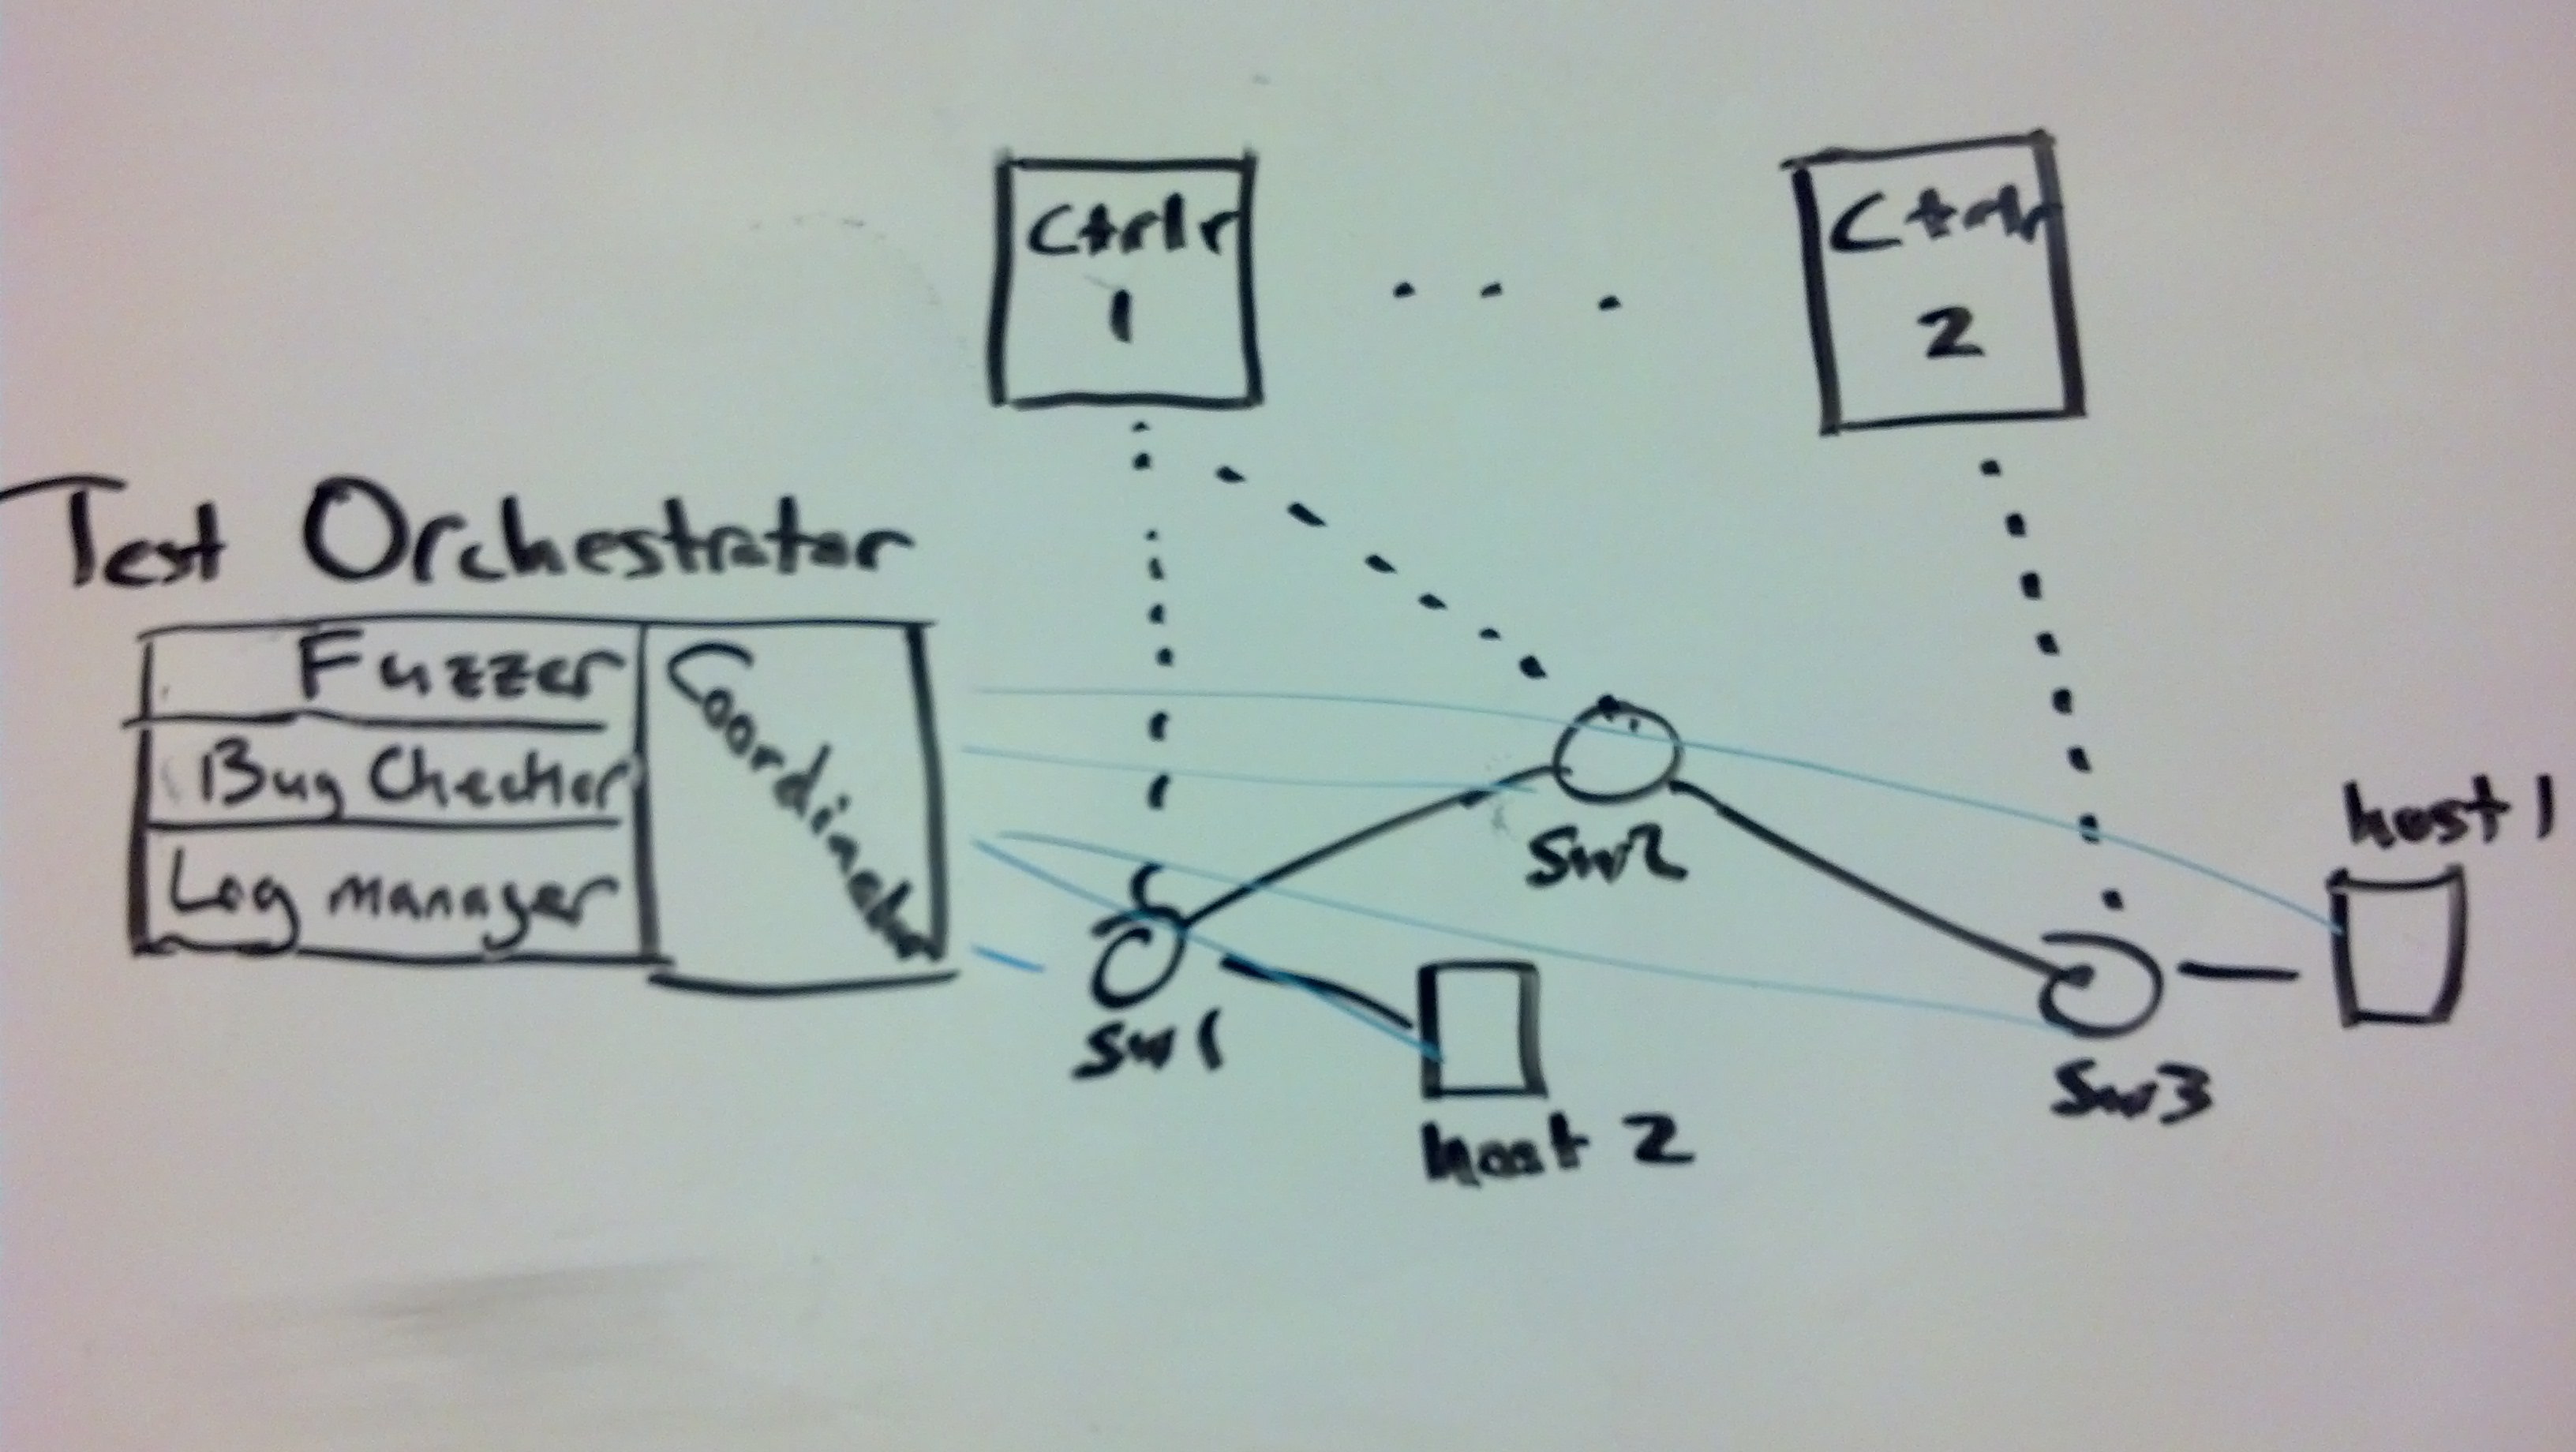
\includegraphics[width=3.25in]{../diagrams/architecture/qa_cluster.jpg}
    \caption[]{\label{fig:qa_cluster} Typical QA testbed. A centralized test
    orchestrator drives the behavior of the network, and checks for bugs in
    the controllers.}
\end{figure}

We do not have access to such a QA testbed.\footnote{If we did have access to
such a QA testbed, we would simply add delta debugging to the test
orchestrator, and potentially insert interposition points throughout the
testbed to enforce causal relations during replay.}
We instead built our own integration testing framework to discover bugs and
perform replay. Our system mocks out the control-plane
behavior of network devices in lightweight software switches and hosts (with
support for minimal data-plane forwarding)
within a single-threaded process. We then run the control software on
top of this simulator and connect the software switches to the controllers as if they were true
network devices, such that the controllers believe they are configuring a true
network. The simulator interposes and buffers messages on all communication
channels, allowing it to delay, drop, or reorder
messages as needed to induce failure modes during testing. During
replay, the simulator uses these buffers to maintain causal dependencies by
matching messages in the buffers by their fingerprints and carefully
controlling the order message are let through according to the subsequence chosen by
delta debugging. The overall simulation architecture is depicted in
Figure~\ref{fig:architecture}.

\begin{figure}[t]
    %\hspace{-10pt}
    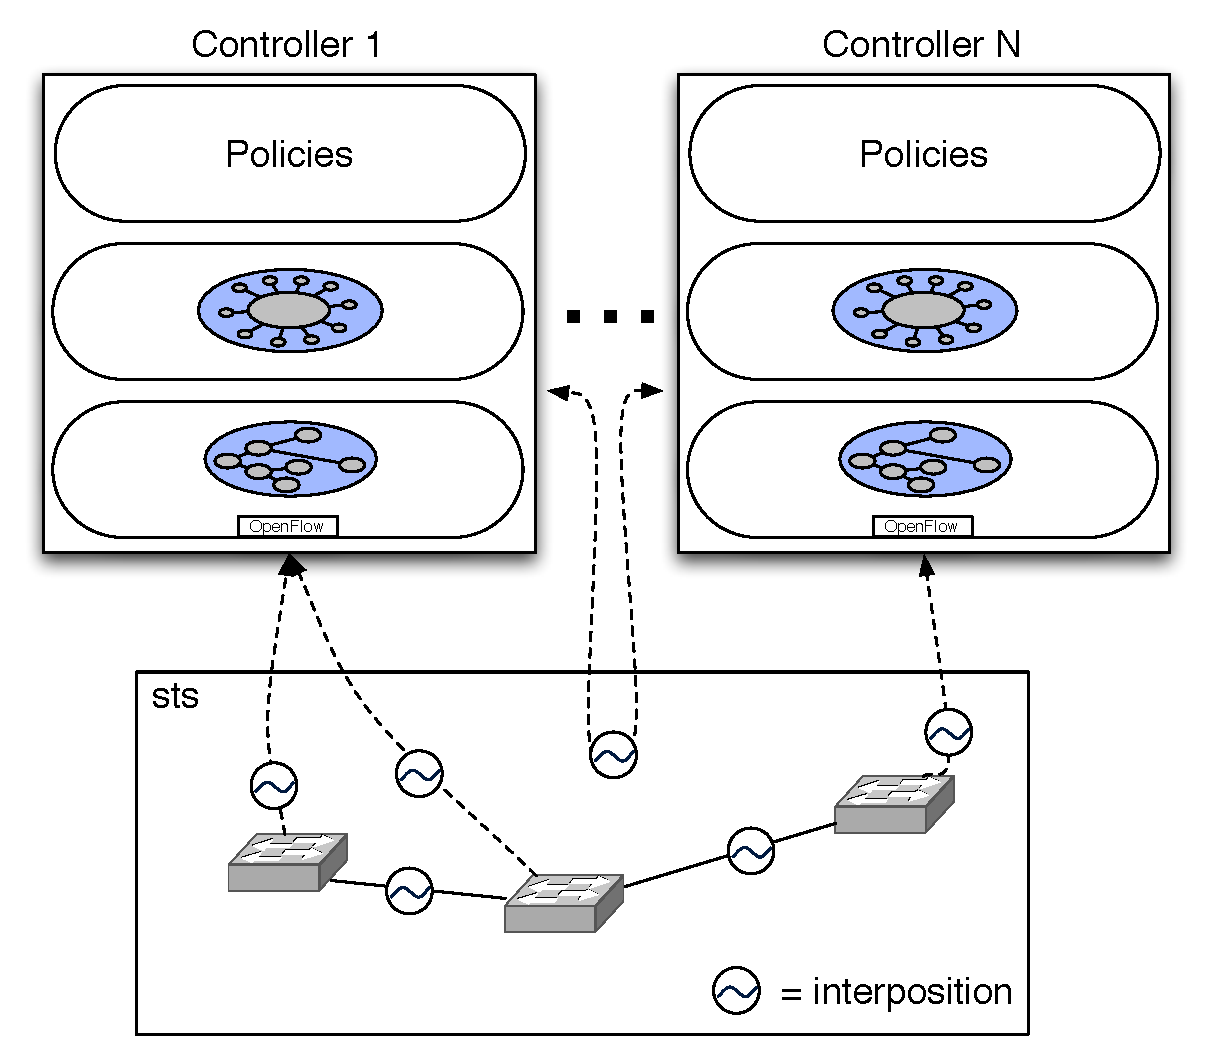
\includegraphics[width=3.25in]{../diagrams/architecture/Debugger_Architecture.pdf}
    \caption[]{\label{fig:architecture} Simulation infrastructure. We simulate
    network devices in software, and interpose on all communication
    channels.}
\end{figure}

\begin{table}
\centering
\begin{tabular}{|l|l|}
\hline
Input Type &  Implementation \\
\hline
\hline
Switch failure/recovery & TCP teardown \\
\hline
Controller failure/recovery & SIGKILL \\
\hline
Link failure/recovery & ofp\_port\_status \\
\hline
Controller partition & iptables \\
\hline
Dataplane packet injection & network namespaces \\
\hline
Dataplane packet drop & dataplane interposition \\
\hline
Dataplane packet delay & dataplane interposition \\
\hline
Host migration & ofp\_port\_status \\
\hline
Control message delay & controlplane interposition \\
\hline
Non-deterministic TCAMs & controlplane interposition \\
\hline
\end{tabular}
\caption{Input types currently supported by \projectname}
\label{tab:inputs}
\end{table}

\begin{table}
\centering
\begin{tabular}{|l|l|}
\hline
All-to-all reachability & Loop freeness \\
\hline
Blackhole freeness & Controller liveness \\
\hline
POX ACL compliance & ONOS flow routing compliance \\
\hline
\end{tabular}
\caption{Invariant checks currently supported by \projectname}
\label{tab:invariants}
\end{table}

We begin by using our simulator to perform testing on controllers to find
bugs. Our most common use case involves generating randomly chosen input
sequences~\cite{Miller:1990:ESR:96267.96279}, feeding them to controller(s),
and monitoring
invariants at chosen intervals.\footnote{The full list of invariants currently
supported is shown in Table~\ref{tab:invariants}}
We also run the simulator interactively
so that we can examine the state of any part of the simulated network,
observe and manipulate messages, and follow our
intuition to induce orderings that we believe may trigger bugs.
Either way, controlling the inputs from a single location
allows the simulator to easily record a global, causally-consistent
event ordering.

After discovering an invariant violation of interest, the simulator replays
the logged sequence of inputs (such as link failures, controller crashes, or host
migrations). For example, the simulator replays link failures
by disconnecting the edge in the simulated network, and sending a
OpenFlow~\cite{openflow} port status message from the adjacent switches to their parent controller(s).

\projectname~(\projectmeaning) is our realization of this simulator.
\projectname~is implemented in roughly 18,000 lines of Python in
addition to the Hassel network invariant checking library~\cite{hsa}.
\projectname~also optionally makes use of Open vSwitch~\cite{pfaff2009extending} as an interposition point for
messages sent between distributed controllers. We have
made the code
for \projectname~publicly available (anonymized), % at \href{http://ucb-sts.github.com/sts}{ucb-sts.github.com/sts},
and have discussed the logistics of deploying it with several SDN companies.

\colin{TODO: Discuss the value of replay for root causing here? Or just let
the use cases speak for themselves?}

%How do we ensure the same scheduling order of controller processes? (see
%Section 4.5 of ReVirt\cite{Dunlap:2002:REI:844128.844148}). We observe that the controllers do not use any shared
%memory communication.}

\subsection{Coping with Non-Determinism}

Non-determinism in the execution of concurrent processes stems from
differences in system call return values, scheduling decisions (which can
even affect the result of individual instructions, such as x86's
interruptable block memory instructions~\cite{Dunlap:2002:REI:844128.844148}), and signal
delivery. These sources of non-determinism may affect whether \projectname~is
able to reproduce the original bug after replay.

Most testing systems, such as the QA testing frameworks we are
trying to improve, do not attempt to mitigate non-determinism; they assume
that developers will be able replicate bugs by attempting to reproduce the
same conditions as the original test run, else track down the the root cause simply by
inspecting the raw execution logs.

\projectname's main approach to coping with non-determinism
is to replay each subsequence chosen
by delta debugging multiple times. If observing the bug
is an independent and identically distributed random variable (an optimistic
but not completely unreasonable assumption) with some
underlying probability $p$, then $n$
replays will observe the bug with probability $1-(1-p)^{n}$. The exponential
works strongly in our favor; for example, even if the original bug is
triggered in only 20\% of replays, the probability that we will not trigger
it during an intermediate replay is approximately
1\% if we replay 20 times per subsequence.

\subsection{Mitigating Non-Determinism}

In cases where non-determinism's effect on replayability is substantial,
one might also seek to mitigate or prevent non-determinism altogether.
Deterministic replay techniques~\cite{Dunlap:2002:REI:844128.844148,Geels:2006:RDD:1267359.1267386},
which precisely record and replay scheduling decisions and system call return values,
may be deployed to reliably produce bugs in exchange for a loss in performance.
Unfortunately these techniques do not allow the user to make any modifications to the processes
involved in the replay. In particular, they do not support changes to the inputs fed to the
processes, since changes may cause the remaining execution to
subtly differ (\eg~the sequence numbers of packets may all differ).
This precludes the possibility of employing deterministic replay techniques in
\projectname, since our goal is precisely to modify the inputs fed to the
distributed system.
%And even if these sources were
%eliminated, it would not be possible to achieve perfectly deterministic
%replay in all cases without full visibility into internal events--a daunting
%instrumentation task.

We therefore designed \projectname~to be as resilient to non-determinism as is
practically feasible, while avoiding modifications to control software whenever possible.
We began by designing \projectname~to run within a single thread, allowing it
to replay all network events in serial order. We also ensured that all
datastructures within \projectname~were not effected by randomness; for example,
we avoid using hashmaps that hash keys according to their memory address,
and sort all list return values.

We also optionally interpose or modify the controller software itself.
Routing the {\tt gettimeofday()} syscall through \projectname~helps ensure that timers fire
at the appropriate point.\footnote{When the pruned trace differs from the original, we make a
best-effort guess at what the return values of these calls should be. For example,
if the altered execution invokes {\tt gettimeofday()} more times than we recorded
in the initial run, we interpolate the time values of neighboring events}
When sending data over multiple sockets, the operating system exhibits
non-determinism in the order it schedules the I/O operations.
\projectname~optionally ensures a deterministic order of messages
by multiplexing all sockets
onto a single true socket. \projectname~currently overrides socket functionality within the control
software itself.\footnote{Only supported for POX at the moment.}
%In the future we plan to implement deterministic message ordering without code modifications by
%loading a shim layer on top of
%libc (similar to liblog~\cite{Geels:2006:RDD:1267359.1267386}).

\projectname~may need visibility into the control software's internal state
changes to reliably reproduce the system execution. We achieve this by
making a
small change to the control software's logging library\footnote{Only supported
for POX and Floodlight at the moment.}: whenever a control process executes a log
statement (which indicate that an important state change is about to take
place), we notify \projectname. We can also use logging interposition as a
synchronization barrier, by blocking the process when it hits crucial logging statements in the code
until \projectname~explicitly tells the process that it may proceed.
%If blocking was enabled
%during recording, we force the control software to block at internal state
%transition points again during replay
%until \projectname~gives explicit acknowledgment.

\subsection{Root Causing Tools}

Tools for root causing, beyond `grep` and the like.

\noindent{\bf OFRewind}:
Sometimes Replayer moves too quickly to get a good understanding of an event
trace. InteractiveReplayer is a combination of Interactive mode and Replayer
mode, a la OFRewind~\cite{ofrewind}.
* visualizing the network topology
* tracing the series of link/switch failures/recoveries
* tracing the series of host migrations
* tracing the series of flow\_mods
* tracing the series of traffic injections
* tracing the series of controller failures, recoveries, and partitions

Each time we hit enter,
the next event in the trace is executed. We can also check invariants, examine
flow tables, visualize the topology, and even induce previously unobserved
inputs.

Because the timing of events is so delicate in a distributed system,
InteractiveReplayer does not run controller processes. Instead, it mocks out
OpenFlow connections, and replays the exact OpenFlow commands from the
original trace.

\noindent{\bf Packet Tracing}:
A la xtrace and ndb~\cite{fonseca2007x,handigol2012debugger}.
It is often useful to know what path a packet took through the network. Given
the event id of a TrafficInjection event, the
script will print all dataplane permits and
drops, as well as ofp\_packet\_in's and out's associated with the
TrafficInjection's packet.

\noindent{\bf OpenFlow analysis}:
The OpenFlow commands sent by controller software are often somewhat redundant. For
example, flow\_mods may override each other, expire, or periodically flush the
contents of flow tables and later repopulate them. Hence even in minimized event
traces we often observe OpenFlow messages that are not directly relevant
for causing an invalid network configuration such as a loop or blackhole.

OpenFlowReplayer mode is designed to filter out such redundant messages,
leaving only the flow\_mods that show up in the final routing tables.
With this knowledge, it becomes much easier to know exactly what points in
the trace the invalid network configuration was installed.
After replaying all OpenFlow commands, OpenFlowReplayer infers which
flow\_mods show up in the final routing tables.

\noindent{\bf Visualization tools}:
Understanding the timing of messages and internal events in distributed systems is a crucial part of troubleshooting.
STS includes two visualization tools designed help with this task.

We include a second visualization tool, `./tools/visualization/visualize1d.html`, to help us compare
the behavior of two or more event traces. This tool is particularly useful for understanding the effects of non-determinism in
intermediate runs of delta debugging.

A common workflow for the trace comparison tool:
- Run MCSFinder.
- Discover that the final MCS does not reliably trigger the bug.
- Open `visualize1D.html` in a web browser.
- Load either the original (fuzzed) trace,
  or the first replay of this trace,
  as the first timeline. I have found that it is often better to load the
  first replay rather than the original fuzzed trace, since this has
  timing information that matches the other replays much more closely.
- Load the final replay of the MCS trace,
  as the second timeline.
- Hover over events to further information about them, including functional equivalence
  with events in the other traces.
- Load intermediate replay trace timelines if needed.

\subsection{Scaling and Parallelization}

When minimizing very large event traces, we found that the python garbage
collector often became overwhelmed (causing the process to slow down
substantially) after replaying several subsequences.
After observing this behavior we modified \projectname~to fork a process
(either local or remote) for each subsequence chosen by delta debugging,
and gather the results of the replay via RPC. This alleviates the slow down,
since the replay process is fully cleaned up by the operating system once the
replay terminates, and the
main delta debugging process keeps little memory itself.
As an added benefit, this architectural change allows us to support
parallelized delta debugging across multiple cores or machines.

\subsection{Enabling Analysis of Production Logs}
\colin{Cut if we need space.}

\projectname~does not currently support minimization of production (as opposed
to QA) logs.
Here we present a sketch of how \projectname~might support production logs as input.

While \simulator~takes as input a single, totally-ordered log of the events in the
distributed system, production systems maintain a log at each node.
Production systems would need to include Lamport
clocks on each message~\cite{Lamport:1978:TCO:359545.359563} or have
sufficiently accurate clock
synchronization~\cite{corbett2012spanner} to obtain a partial global ordering
consistent with the happens-before relation.\footnote{
Note that a total ordering is not needed, since it is permissible
for \simulator~to reorder concurrent events from
the production run so long as the happens-before relation is
maintained~\cite{Fischer:1985:IDC:3149.214121}.}
Inputs would also need to need to be logged in sufficient detail for \projectname~to
replay a synthetic version of the input that is indistinguishable (in terms
of control plane messages) from the original.

Without care, a single input event may appear multiple times in the
distributed logs. A failure of the master node, for example, could be independently
detected and logged by all other replicas. The most robust way to
avoid redundant input events would be to employ perfect failure
detectors~\cite{chandra1996unreliable}, which log a failure iff
the failure actually occurred.\footnote{Perfect failure detectors can be
implemented in partially synchronous distributed systems by explicitly killing
nodes that are suspected to be down.} % Ensuring that a single failure detector is in charge of logging node failure
% events guarantees that redundant events do not appear.
Alternatively, one
could employ root cause analysis
algorithms~\cite{yemini1996} or manual inspection to consolidate redundant
alarms.

Finally, some care would be needed to prevent the logs from growing so large that
\simulator's runtime becomes intractable. Here, causally consistent
snapshots~\cite{Chandy:1985:DSD:214451.214456} would allow \projectname~to
bootstrap its simulation from the last snapshot before the failure rather than
replaying from the beginning of the log.
%If the MCS starting from this snapshot is empty, it could iteratively move backwards, starting from earlier
%snapshots.

\subsection{Limitations}
\label{subsec:non_goals}

Having detailed the specifics of our approach we now
clarify the scope of our technique's use.

\noindent{\bf Partial Visibility.} Our event scheduling algorithm assumes that
it has visibility into the occurrence of all relevant internal events. This
may involve substantial instrumentation effort beyond
pre-existing log statements.

\noindent{\bf Non-determinism Within Individual Controllers.} Non-determinism
is fundamental in networks. We try our best to mitigate and cope with
non-determinism, but it may be so bad that bugs are reproducibility. In
particular our technique is not designed to reproduce bugs
involving non-determinism within a single controller (\eg~race-conditions between threads);
we focus on coarser granularity errors (\eg~incorrect failover logic). Nonetheless, the
worst case for us is that the developer ends up with what they started:
an unpruned log.

%The upshot of
%this is that our technique is not able to minimize all possible failures.
%Nonetheless, our worst case is that the developer ends up with what they started:
%an unpruned log.

\eat{That said, if the developer is willing to instrument their system to
provide finer granularity log messages (\cf~\cite{Geels:2006:RDD:1267359.1267386}),
our approach readily supports deterministic replay.}

\eat{
\noindent{\bf Troubleshooting vs.\ Debugging.} Our technique is a troubleshooting tool, not a debugger;
by this we mean that our approach helps identify and localize inputs that
trigger erroneous behavior, but it does not directly identify which
line(s) of code cause the error.}

\noindent{\bf Bugs Outside the Control Software.} Our goal is not to find the root
cause of individual component failures in the system (\eg~misbehaving routers,
link failures). Instead, we focus on
how the distributed system as a whole reacts to the occurrence of such inputs.
%If there is a bug in your switch, you will need to contact your hardware vendor;
%if you have a bug in your policy specification, you will need to take a closer look at what you specified.

\noindent{\bf Globally vs.\ Locally Minimal Input Sequences.}
Our approach is not guaranteed to find the globally minimal
causal sequence from an input trace, since this enumerating the powerset of
$E_L$ in the worst case (a $O(2^n)$ operation).
The delta debugging algorithm we employ does provably find a
locally minimal causal sequence~\cite{Zeller:1999:YMP:318773.318946},
meaning that if any input from the sequence is pruned, no invariant violation
occurs.

\noindent{\bf Correctness vs.\ Performance.}
We are primarily focused on correctness bugs, not performance bugs.

\noindent{\bf Bugs Found Through Fuzzing.}
We generate bug traces primarily through fuzz testing, not from real bugs
found in operation. There is a substantial practical hurdle in instrumenting
operational systems to produce logs that can be injected into our system. % , and we have not addressed those issues yet.
%In practice some bugs
%found through fuzzing will not be considered worthwhile to investigate.

\noindent{\bf Scaling.}
Our discussions with companies with large SDN deployments suggest that scaling to the size of the
large logs they collect will be a substantial challenge.
On the other hand, the fact that these logs are so large makes the need for finding MCSes even more acute.

\eat{
\noindent{\bf Proactive vs.\ Reactive Configuration.} We focus primarily on
\emph{proactive} configuration, where controllers react to policy and topology changes, but
not necessarily individual packets or flows events in the
dataplane.\footnote{Production controllers typically adopt this model for
performance reasons.}
The main challenge in extending our approach to reactive controllers is
achieving efficient simulation of dataplane traffic.
\andi{Could cut this. We actually find reactive bugs}
}

